\documentclass[aspectratio=169]{../latex_main/tntbeamer}  % you can pass all options of the beamer class, e.g., 'handout' or 'aspectratio=43'
\usepackage{dsfont}
\usepackage{bm}
\usepackage[english]{babel}
\usepackage[T1]{fontenc}
%\usepackage[utf8]{inputenc}
\usepackage{graphicx}
\graphicspath{ {./figures/} }
\usepackage{algorithm}
\usepackage[ruled,vlined,algo2e,linesnumbered]{algorithm2e}
\usepackage{hyperref}
\usepackage{booktabs}
\usepackage{mathtools}

\usepackage{amsmath,amssymb}

\DeclareMathOperator*{\argmax}{arg\,max}
\DeclareMathOperator*{\argmin}{arg\,min}

\usepackage{pgfplots}
\pgfplotsset{compat=1.16}
\usepackage{tikz}
\usetikzlibrary{trees} 
\usetikzlibrary{shapes.geometric}
\usetikzlibrary{positioning,shapes,shadows,arrows,calc,mindmap}
\usetikzlibrary{positioning,fadings,through}
\usetikzlibrary{decorations.pathreplacing}
\usetikzlibrary{intersections}
\pgfdeclarelayer{background}
\pgfdeclarelayer{foreground}
\pgfsetlayers{background,main,foreground}
\tikzstyle{activity}=[rectangle, draw=black, rounded corners, text centered, text width=8em]
\tikzstyle{data}=[rectangle, draw=black, text centered, text width=8em]
\tikzstyle{myarrow}=[->, thick, draw=black]

% Define the layers to draw the diagram
\pgfdeclarelayer{background}
\pgfdeclarelayer{foreground}
\pgfsetlayers{background,main,foreground}

% Requires XeLaTeX or LuaLaTeX
\usepackage{unicode-math}

\usepackage{fontspec}
%\setsansfont{Arial}
\setsansfont{RotisSansSerifStd}[ 
Path=../latex_main/fonts/,
Extension = .otf,
UprightFont = *-Regular,  % or *-Light
BoldFont = *-ExtraBold,  % or *-Bold
ItalicFont = *-Italic
]
\setmonofont{Cascadia Mono}[
Scale=0.8
]

% scale factor adapted; mathrm font added (Benjamin Spitschan @TNT, 2021-06-01)
%\setmathfont[Scale=1.05]{Libertinus Math}
%\setmathrm[Scale=1.05]{Libertinus Math}

% other available math fonts are (not exhaustive)
% Latin Modern Math
% XITS Math
% Libertinus Math
% Asana Math
% Fira Math
% TeX Gyre Pagella Math
% TeX Gyre Bonum Math
% TeX Gyre Schola Math
% TeX Gyre Termes Math

% Literature References
\newcommand{\lit}[2]{\href{#2}{\footnotesize\color{black!60}[#1]}}

%%% Beamer Customization
%----------------------------------------------------------------------
% (Don't) Show sections in frame header. Options: 'sections', 'sections light', empty
\setbeamertemplate{headline}{empty}

% Add header logo for normal frames
\setheaderimage{
	% 
\includegraphics[height=\logoheight]{figures/TNT_darkv4.pdf}
	
\includegraphics[height=\logoheight]{../latex_main/figures/luh_logo_rgb_0_80_155.pdf}
	% 
\includegraphics[height=\logoheight]{figures/logo_tntluh.pdf}
}

% Header logo for title page
\settitleheaderimage{
	% 
\includegraphics[height=\logoheight]{figures/TNT_darkv4.pdf}
	
\includegraphics[height=\logoheight]{../latex_main/figures/luh_logo_rgb_0_80_155.pdf}
	% 
\includegraphics[height=\logoheight]{figures/logo_tntluh.pdf}
}

% Title page: tntdefault 
\setbeamertemplate{title page}[tntdefault]  % or luhstyle
% Add optional title image here
%\addtitlepageimagedefault{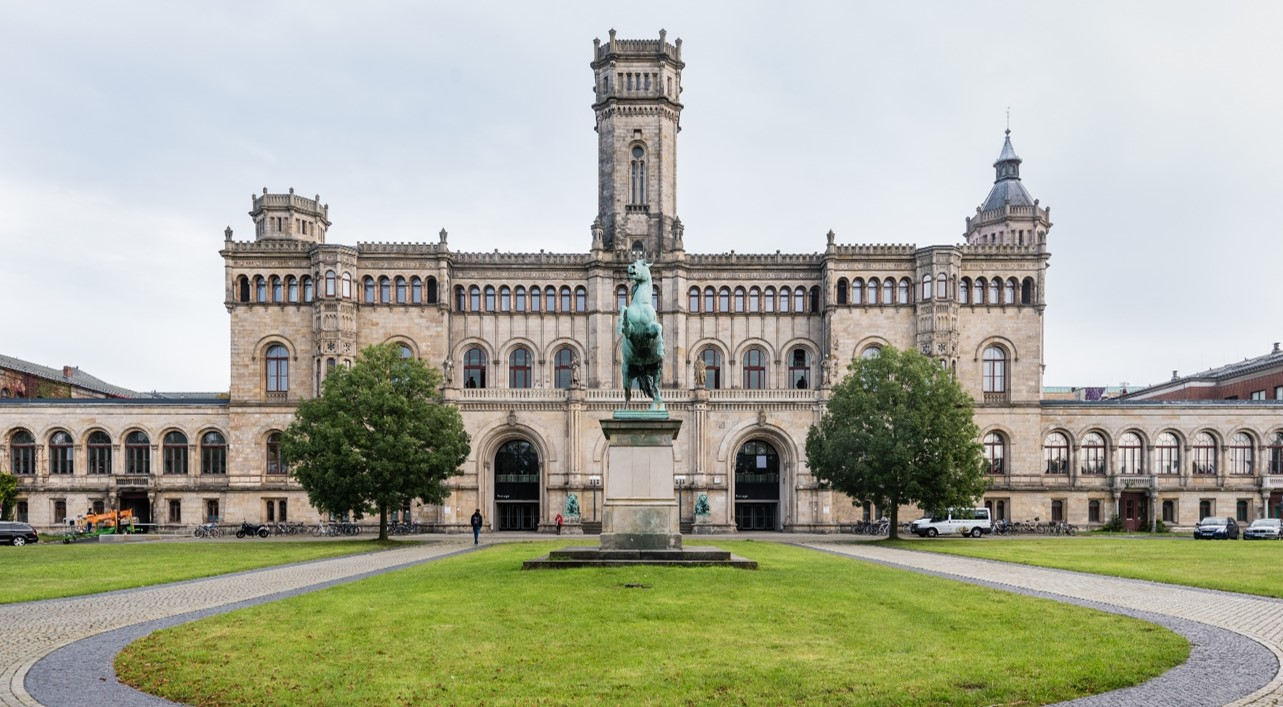
\includegraphics[width=0.65\textwidth]{figures/luh_default_presentation_title_image.jpg}}

% Title page: luhstyle
% \setbeamertemplate{title page}[luhstyle]
% % Add optional title image here
% \addtitlepageimage{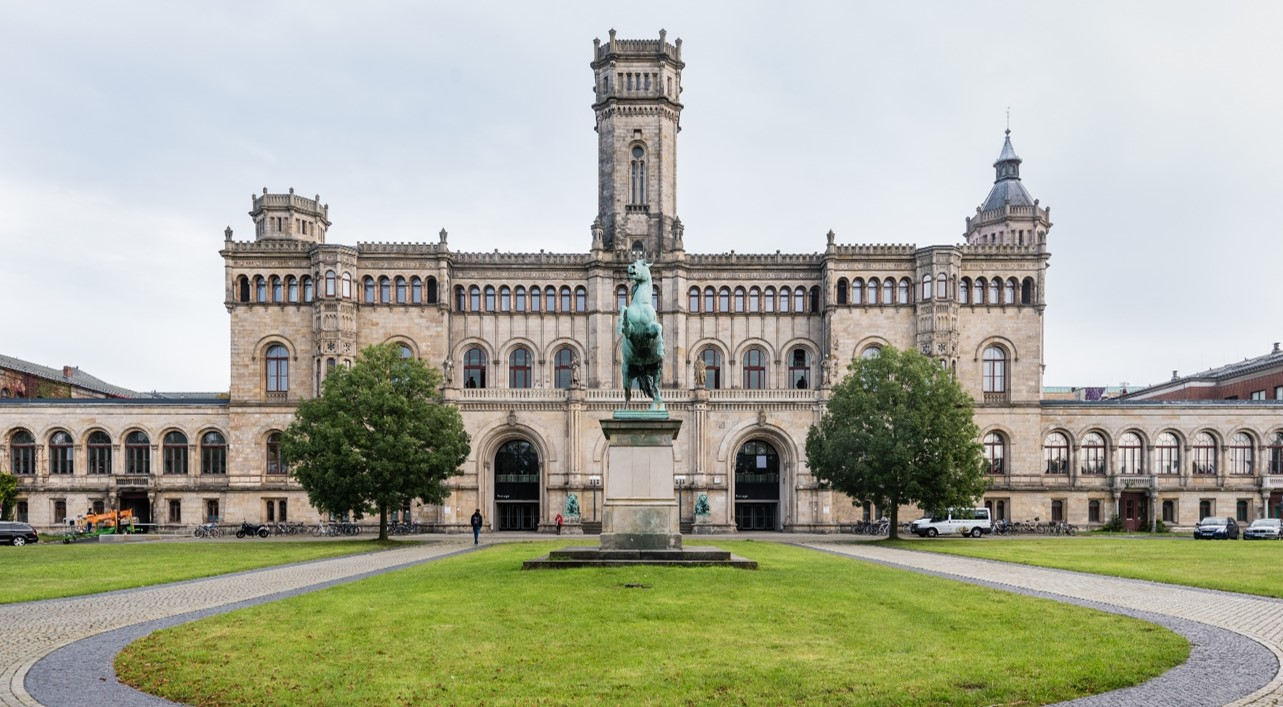
\includegraphics[width=0.75\textwidth]{figures/luh_default_presentation_title_image.jpg}}

\author[Lindauer \& Anand]{Marius Lindauer and Avishek Anand\\[1em]
	
\includegraphics[height=\logoheight]{../latex_main/figures/luh_logo_rgb_0_80_155.pdf}\qquad

\includegraphics[height=\logoheight]{../latex_main/figures/TNT_darkv4}\qquad

\includegraphics[height=\logoheight]{../latex_main/figures/L3S.jpg}	}
\date{Winter Term 2021
}


%%% Custom Packages
%----------------------------------------------------------------------
% Create dummy content
\usepackage{blindtext}

% Adds a frame with the current page layout. Just call \layout inside of a frame.
\usepackage{layout}


\title[Introduction]{iML: Introduction}
\subtitle{Permutation Feature Importance}
%\institute{}
\newcommand{\predvar}{Var\left[\hat{f}(x)\right]}


\begin{document}
	
	\maketitle

\begin{frame}{Permutation Feature Importance \lit{Fischer et al. 2018}{https://arxiv.org/abs/1801.01489}}
\textbf{Idea:} Permuting a feature breaks the association between the feature and the target.\\
\smallskip\pause
$\Rightarrow$ Model's prediction error should increase after permutation if the considered feature is important.

\pause
\begin{figure}
  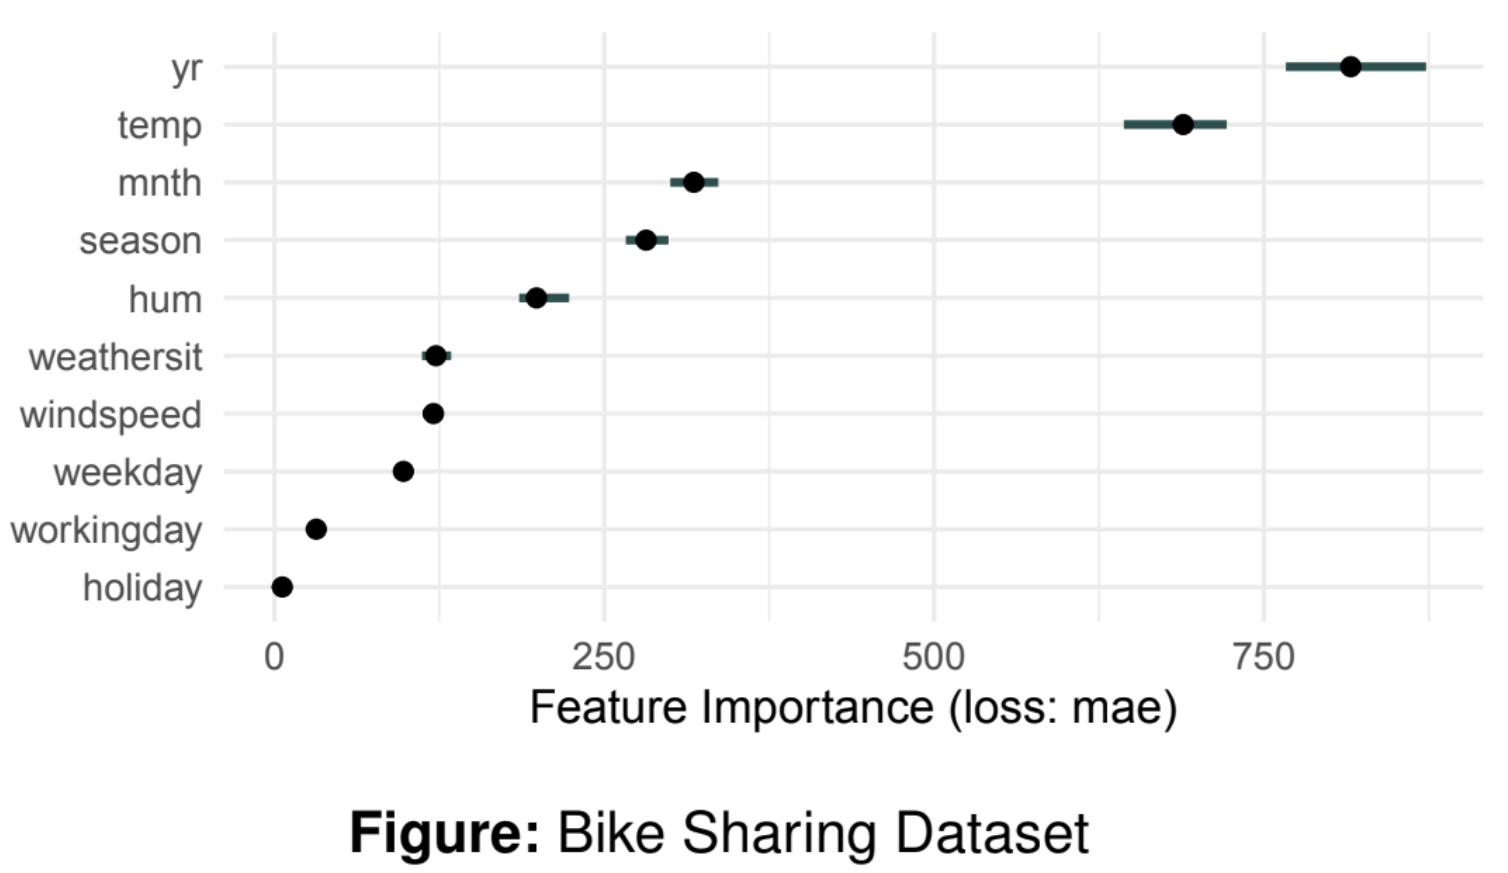
\includegraphics[width=0.7\textwidth]{figure/feature-importance.png}
\end{figure}

\end{frame}

\begin{frame}{Permutation Feature Importance}

Performance-based permutation feature importance (PFI) for a feature $x_S$ using test data $\mathcal{D}$:
\begin{itemize}
  \item Measure the error \color{red}\textbf{with permuted feature values} \color{black} for $x_S$.
  \item Measure the error \color{blue}\textbf{without permuting features}\color{black}.
  \item Repeat permuting the feature (e.g., $m$ times) and average the difference of both errors: 
$$\widehat{PFI}_S = \frac{1}{m} \sum_{k = 1}^{m} \widehat{GE}(\hat{f}, {\color{red}\mathcal{D}_{S}^{(k)}}) - \widehat{GE}(\hat{f}, {\color{blue}\mathcal{D}})$$
\end{itemize}

Example of permuting feature $x_S$ with $S = \{1\}$:

\begin{center}
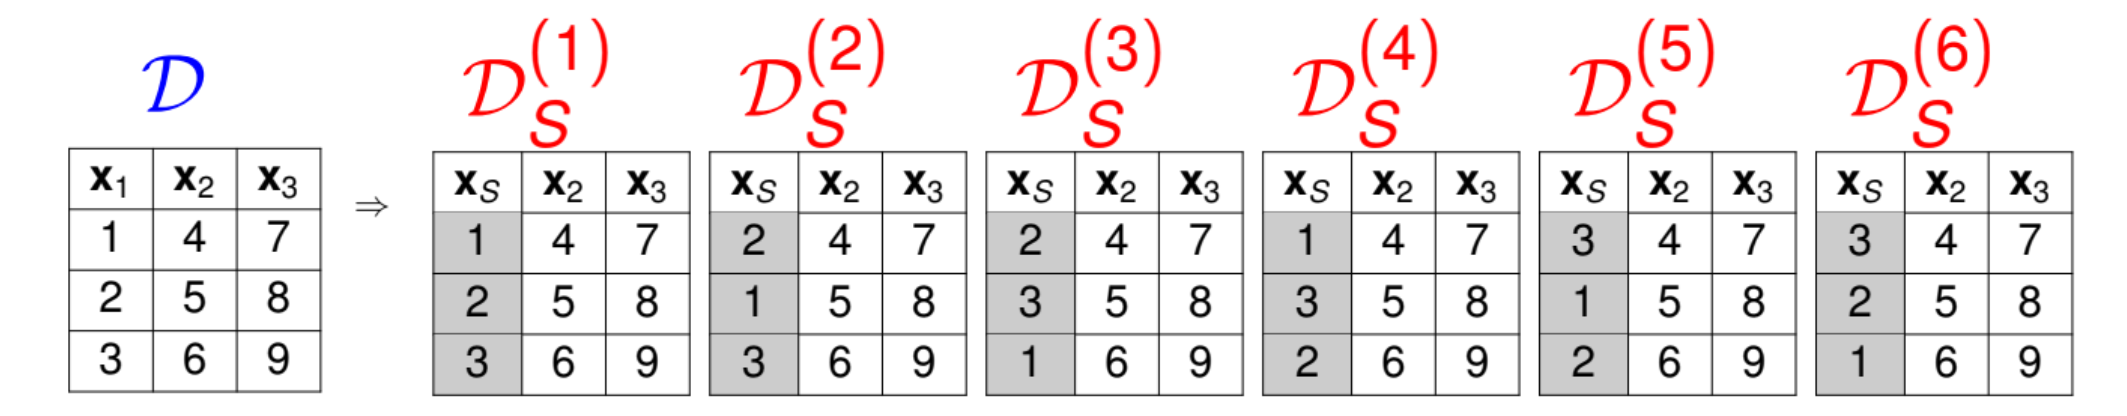
\includegraphics[width=0.75\textwidth]{figure/permuted-fv.png}
\end{center}

% \vspace*{0.2cm}
% {\scriptsize{Note: 
% The $S$ in $x_S$ refers to a \textbf{S}ubset of features for which we are interested in their effect on the prediction.
% As we calculate the feature importance for one feature at a time $|S| = 1$.}\par}

\end{frame}
\begin{frame}{Permutation Feature Importance}

Steps to calculate the PFI for a single feature $x_S$ according to the SIPA framework:
\begin{enumerate}
  \item \textbf{Sampling:} Sample feature values from the distribution of $x_S$. \newline $\Rightarrow$ Randomly permute feature $x_S$ (retains the distribution).
  \item \textbf{Intervention:} Replace the original feature of the test dataset $\mathcal{D}$  with the permuted feature  creating the dataset $\mathcal{D}_{S}$.
  \item \textbf{Prediction:} Make predictions for both data, i.e., $\mathcal{D}$ and $\mathcal{D}_{S}$.
  \item \textbf{Aggregation:} 
    \begin{itemize}
      \item Compute the loss for each observation in both data sets.
      \item Take the difference of both losses $\Delta L$ for each observation.
      \item Average this change in loss across all observations.
      \item Also, average over multiple repetitions, if available.
    \end{itemize}
\end{enumerate}
\end{frame}


\frame{

\frametitle{Permutation Feature Importance}
    \vspace{-1em}
    
  {\hspace{2em}\only<1-3,5-7>{$\hspace{36pt}{\color{white}\widehat{GE}(\hat{f}, {\color{red}\mathcal{D}_{S}^{(k)}}) - \widehat{GE}(\hat{f}, {\color{blue}\mathcal{D}})}$}
  \only<4>{$\hspace{36pt}\widehat{GE}(\hat{f}, {\color{red}\mathcal{D}_{S}^{(k)}}) - \widehat{GE}(\hat{f}, {\color{blue}\mathcal{D}}),$ where 
$\scriptstyle\widehat{GE}(\hat{f}, \mathcal{D}) =$ \scalebox{0.7}{$\frac{1}{n} \sum\nolimits_{(x, y) \in \mathcal{D}}$} $\scriptstyle L(\hat{f}(x), y)$}}
% $\scriptstyle\widehat{GE}(\hat{f}, \mathcal{D}) =$ \scalebox{0.7}{$\frac{1}{n} \sum\nolimits_{(x, y) \in \D}$} $\scriptstyle L(\hat{f}(x), y)$}
%   \only<5-6>{$\hspace{36pt}{\color{white}\widehat{GE}(\hat{f}, {\color{red}\mathcal{D}_{S}^{(k)}}) - \widehat{GE}(\hat{f}, {\color{blue}\mathcal{D}})}$}
  
  \begin{center}
  \only<1>{\includegraphics[page=2, trim=0pt 5pt 0 66pt, clip, width=0.58\textwidth]{figure/pfi_demo2}}%
  \only<2>{\includegraphics[page=3, trim=0pt 5pt 0 66pt, clip, width=0.58\textwidth]{figure/pfi_demo2}}%
  \only<3-4>{\includegraphics[page=4, trim=0pt 5pt 0 66pt, clip, width=0.58\textwidth]{figure/pfi_demo2}}%
  \only<5>{\includegraphics[page=5, trim=0pt 5pt 0 66pt, clip, width=0.58\textwidth]{figure/pfi_demo2}}%
  \only<6>{\includegraphics[page=6, trim=0pt 5pt 0 66pt, clip, width=0.58\textwidth]{figure/pfi_demo2}}%
  \only<7>{\includegraphics[page=7, trim=0pt 5pt 0 66pt, clip, width=0.58\textwidth]{figure/pfi_demo2}}%
  \end{center}
  
  \begin{itemize}
    \only<1-2>{\item[1.]\textbf{Sampling:} Sample feature values from the distribution of $x_S$. \newline $\Rightarrow$ Randomly permute feature $x_S$ (retains the distribution).
        \item[2.] \textbf{Intervention:} Replace the original feature with the permuted feature and create data with permuted feature   $\mathcal{D}_{S}$.}
    \only<2>{\item[3.] \textbf{Prediction:} Make predictions for both data, i.e., $\mathcal{D}$ and $\mathcal{D}_{S}$.}
    \only<3-4>{\item[4.] \textbf{Aggregation:}
      \begin{itemize}
        \item Compute the loss for each observation in both data sets.
      \end{itemize}}
    \only<5>{\item[4.] \textbf{Aggregation:}
      \begin{itemize}
        \item Compute the loss for each observation in both data sets.
       \item Take the difference of both losses $\Delta L$ for each observation.
      \end{itemize}}
     \only<6>{\item[4.] \textbf{Aggregation:}
      \begin{itemize}
        \item Compute the loss for each observation in both data sets.
        \item Take the difference of both losses $\Delta L$ for each observation.
        \item Average this change in loss across all observations.
      \end{itemize}}
    \only<7>{\item[4.] \textbf{Aggregation:}
      \begin{itemize}
        \item Compute the loss for each observation in both data sets.
        \item Take the difference of both losses $\Delta L$ for each observation.
        \item Average this change in loss across all observations.
        \item Also, average over multiple repetitions, if available.
      \end{itemize}}
  \end{itemize}
}

\begin{frame}{Bike Sharing Dataset}

\begin{center}
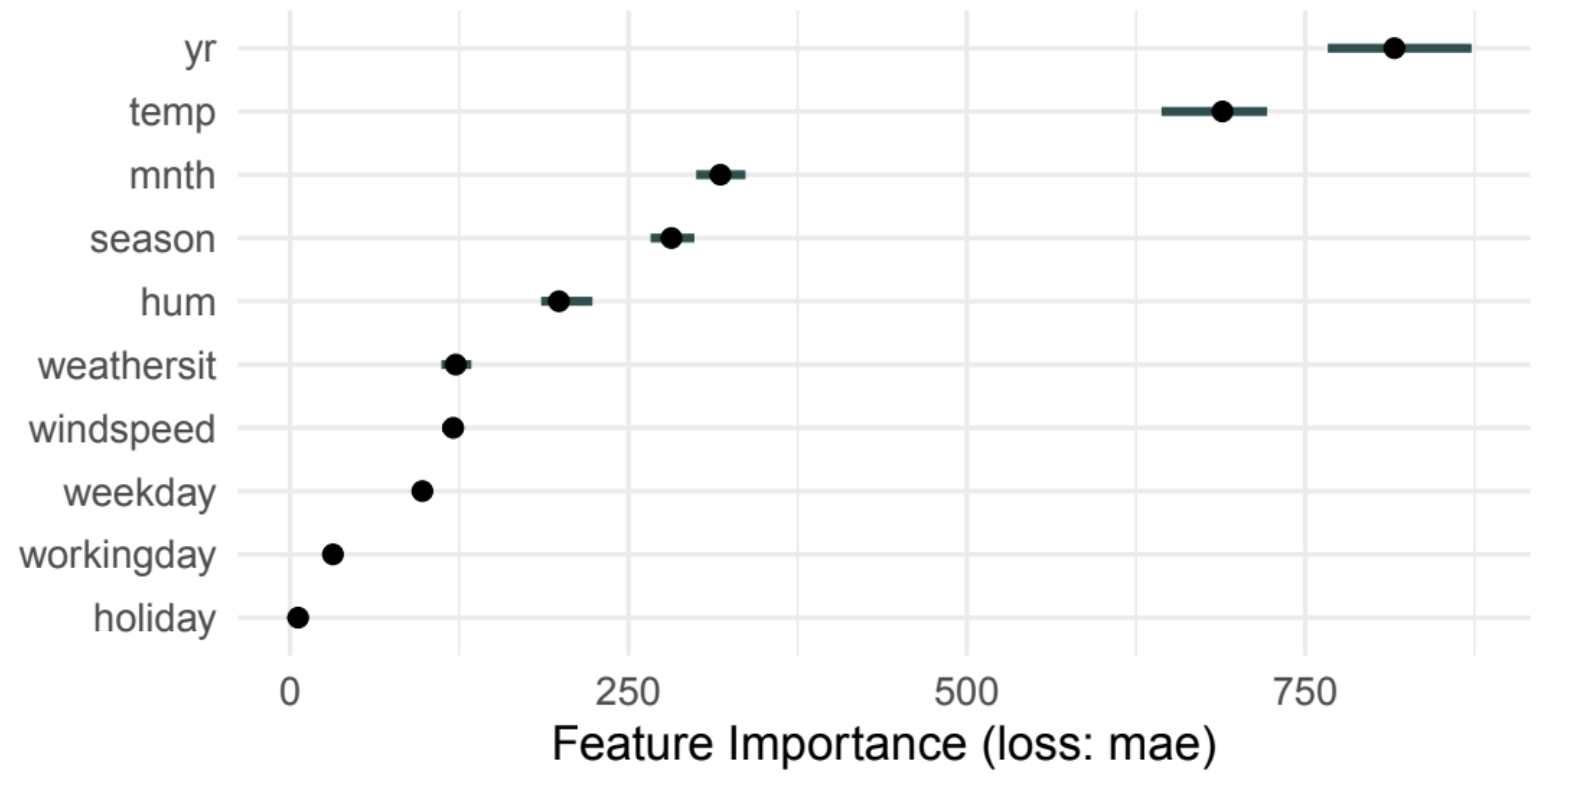
\includegraphics[width=0.5\textwidth]{figure/bike-sharing02.png}
\end{center}

\begin{itemize}
 \item The year is the most important feature.
 \item Destroying the information in ``year'' by shuffling it increases the MAE by 816.
 \item The $5 \%$ and $95 \%$ quantile of the repetitions are shown as error bars.
\end{itemize}
\end{frame}

\begin{frame}{Permutation Feature Importance (PFI)}
 \begin{itemize}
 \itemsep1em
  \item Interpretation: PFI displays the increase of the model error\\ when the feature's information is destroyed.
  \pause
  \item PFI produces a single importance value per feature. \\
  $\leadsto$ It is a global interpretability method.
  \pause
  \item Results can be unreliable due to random permutations. \\
  $\leadsto$ Solution: Average results over multiple repetitions.
  \pause
  \item Disadvantage: Permuting features despite correlation with other features can lead to unrealistic combinations of feature values.
  \pause
  \item Disadvantage: Feature importance automatically includes the importance of interaction effects with other features.
 \end{itemize}
\end{frame}


% \begin{frame}{Testing Importance (PIMP)}

% \begin{itemize}
%   \item PIMP was originally introduced for random forest feature importance.
%   \item It fixes the problem that the importance measure prefers features with many categories.
%   \item PIMP answers the questions when the importance significantly differs from 0. 
%   \item It computes the distribution of importances under the $H_0$-hypothesis that the feature has no influence.
%   \item Sampling under $H_0$ is achieved by permuting the $\ydat$-vector and retraining the model.
%   \item We now rescale the importance to a p-value - the tail probability under $H_0$ - as a new importance score. 
% \end{itemize}

% {\tiny{Altmann, André, et al. "Permutation importance: a corrected feature importance measure." 
% Bioinformatics 26.10 (2010): 1340-134.}}

% \framebreak

% PIMP algorithm:
% \begin{enumerate}
% 	\item For $m \in \{1, \ldots, n_{repetitions}\}$:
% 		\begin{itemize}
% 			\item Permute response vector $\ydat$.
% 			\item Retrain model with data $\Xmat$ and permuted $\ydat$.
% 			\item Compute feature importance $PFI_j^m$ for each feature $j$.
% 		\end{itemize}
% 	\item Train model with $\Xmat$ and unpermuted $\ydat$.
% 	\item For each feature $j \in \{1,\ldots,p\}$:
% 		\begin{itemize}
% 			\item Fit probability distribution of the feature importance values $PFI_j^m$, $m \in \{1, \ldots, n_{repetitions}\}$ (choice between Gaussian, lognormal, gamma or non-parametric).
% 			\item Compute permutation feature importance $PFI_j$ for the model without permutation.
% 			\item Retrieve the p-value of $PFI_j$ based on the fitted distribution.
% 		\end{itemize}
% \end{enumerate}
% \end{frame}



\end{document}
